\section[1977年高考数学试卷(天津卷)理科]{1977年普通高等学校招生考试(天津卷)\\\Huge 数学试卷}

\begin{questions}
	\question
	\begin{parts}
		\part 在什么条件下,$\dfrac{y}{2x}$
			\begin{cenum}
				\item 是正数;
				\item 是负数;
				\item 等于零;
				\item 没有意义?
			\end{cenum}

			\begin{solution}
				\begin{cenum}
					\item $xy>0$;
					\item $xy<0$;
					\item $y=0$且$x\neq 0$;
					\item $x=0$
				\end{cenum}
			\end{solution}

		\part 比较下列各组数的大小,并说明理由.
			\begin{cenum}
				\item $\cos\ang{31}$与$\cos\ang{30}$.
				      \begin{solution}
					      \begin{center}
						      \begin{tikzpicture}
							      \begin{axis}[
									      xmin = -pi/2, xmax = 2.5*pi,
									      ymin = -1.5, ymax = 1.5,
								      ]
								      \addplot[domain=0:2*pi]{cos(deg(x))};
								      \addlegendentry{$\cos(x)$}

								      \node[above] at ({pi/2},0) {$\frac{\pi}{2}$};
							      \end{axis}
						      \end{tikzpicture}
					      \end{center}
					      可以看到余弦函数在第一象限是单调递减的,所以$\cos\ang{31} < \cos\ang{30}$.

				      \end{solution}
				\item $\log_21$与$\log_2\frac14$.
				      \begin{solution}
					      对二者分别求值:
					      \begin{align*}
						      \log_21 = \log_2{2^0} = 0 \\
						      \log_2{\frac14} = \log_2{2^{-2}} = -2
					      \end{align*}
					      所以有$\log_21 > \log_2{\frac14}$.
				      \end{solution}
			\end{cenum}
		\part 求值:
			\begin{cenum}
				\item $\tan \left( 5\arcsin\frac{\sqrt{3}}{2} \right)$.
				      \begin{solution}
					      \begin{align*}
						       & = \tan \left( 5\times \frac{\pi}{3} \right) \\
						       & = \tan \left( \frac{5\pi}{3} \right)        \\
						       & = -\sqrt{3}
					      \end{align*}
				      \end{solution}
				\item $(-2)^0 \times (0.01)^\frac12$.
				      \begin{solution}
					      \begin{align*}
						       & = 1 \times 10^{-2\times\frac12} \\
						       & = 0.1
					      \end{align*}
				      \end{solution}
			\end{cenum}
		\part 计算:$\lg12.5-\lg\frac58+\lg\sin\ang{30}$.
			\begin{solution}
				\begin{align*}
					 & = \lg\frac{25}{2} - \lg\frac58 + \lg\frac12               \\
					 & = \lg \left( \frac{25}{2}\cdot\frac85\cdot\frac12 \right) \\
					 & = \lg10                                                   \\
					 & = 1
				\end{align*}
			\end{solution}

		\part 解方程:
			\begin{math}
				\frac{4x}{x^2-4} - \frac2{x-2} = 1 - \frac1{x+2}.
			\end{math}

			\begin{solution}
				两边同乘以$x^2 - 4, (x\neq\pm2)$得:
				\begin{equation*}
					4x - 2(x+2) = x^2 - 4 - (x-2)
				\end{equation*}
				整理得:
				\begin{equation*}
					x^2 -3x + 2 = 0
				\end{equation*}
				分解因式得:
				\begin{equation*}
					(x-2)(x-1) = 0
				\end{equation*}
				因为$x\neq\pm2$,所以$x=1$.
			\end{solution}

	\end{parts}

	\question
	\begin{parts}
		\part
			某工厂准备在仓库的一侧建立一个矩形储料场(如图),现有$50$米长的铁丝网,如果用它来围成这个储料场,那么长和宽各是多少时,这个储料场的面积最大?并求出这个最大的面积.
			\begin{center}
				\begin{tikzpicture}
					\draw[very thick](0,1) -| (1,.2) (0,-1) -| (1,-.2);
					\draw[thin](1,.7) -| (3, -.7) -- (1,-.7);

					\node at (.5,0){仓库};
					\node at (2,0){储料场};
					\node at (2, -1) {$x$};
					\node[right] at (3, 0) {$y$};
				\end{tikzpicture}
			\end{center}

			\begin{solution}
				面积可以表示成:
				\begin{align*}
					S & = xy          \\
					  & = x(50-2x)    \\
					  & = -2x^2 + 50x
				\end{align*}
				根据抛物线的性质,在$-\frac{b}{2a}=\frac{25}{2}$处面积有最大值,代入面积公式得:
				\begin{equation*}
					S_{max} = \frac{25}{2}(50 - 2\times\frac{25}2) = \qty{312.5}{\meter\squared}
				\end{equation*}
			\end{solution}

		\part 如图,已知$AB$、$DE$是圆$O$的直径,$AC$是弦,$AC\parallel DE$,求证:$CE=EB$.
			\begin{center}
				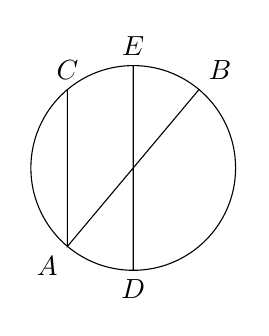
\begin{tikzpicture}[scale=1.3]
					\draw (0,0) circle (1);
					\draw (0,1) -- (0,-1) (50:1) -- (230:1) -- (130:1);

					\node[above] at (0,1) {$E$};
					\node[below] at (0,-1) {$D$};
					\node[above right] at (50:1) {$B$};
					\node[below left] at (230:1) {$A$};
					\node[above] at (130:1) {$C$};
				\end{tikzpicture}
			\end{center}

			\begin{proofsolution}
				\begin{center}
					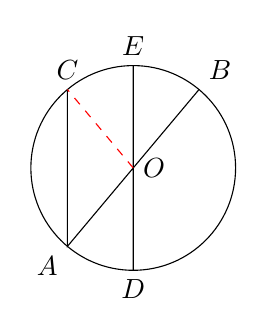
\begin{tikzpicture}[scale=1.3]
						\draw (0,0) circle (1);
						\draw (0,1) -- (0,-1) (50:1) -- (230:1) -- (130:1);

						\node[above] at (0,1) {$E$};
						\node[below] at (0,-1) {$D$};
						\node[above right] at (50:1) {$B$};
						\node[below left] at (230:1) {$A$};
						\node[above] at (130:1) {$C$};

						\draw[dashed, red](0,0) -- (130:1);
						\node[right] at (0,0) {$O$};
					\end{tikzpicture}
				\end{center}
				\begin{cenum}
					\item 连接圆心$O$和$C$点;
					\item
					      \begin{align*}
						       & \because CO = AO                                                 \\
						       & \therefore \angle{A} = \angle{C}                                 \\
						       & \because AC \parallel ED                                         \\
						       & \therefore \angle{C} = \angle{COE} \land \angle{A} = \angle{EOB} \\
						       & \therefore \angle{COE} = \angle{EOB}                             \\
						       & \therefore CE = EB
					      \end{align*}
				\end{cenum}
			\end{proofsolution}
	\end{parts}

	\question 如果已知$bx^2 - 4bx + 2(a+c) = 0\quad (b\neq0)$有两个相等的实数根,求证:$a,b,c$成等差数列.
	\begin{proofsolution}
		因为方程有两个相等的实数根,所以其判别式$\Delta=0$:
		\begin{align*}
			16b^2 - 8b(a+c) = 0 \\
			2b = a+ c           \\
			b - a = c - b
		\end{align*}
		所以$a,b,c$成等差数列.
	\end{proofsolution}

	\question
	\begin{parts}
		\part
			如图,为求河对岸某建筑的高$AB$,在地面上引一条基线$CD=a$,测得$\angle{ACB}=\alpha,\angle{BCD}=\beta,\angle{BDC=\gamma}$,求$AB$.

			\begin{center}
				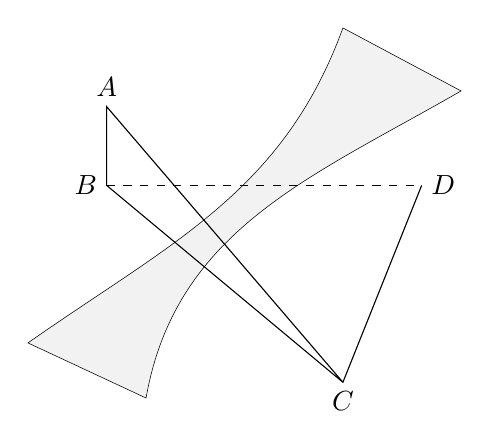
\begin{tikzpicture}
					\coordinate(A) at (0,1);
					\coordinate(B) at (0,0);
					\coordinate(C) at (3,-2.5);
					\coordinate(D) at (4,0);
					\draw[fill=gray!10, very thin](3,2) -- (4.5,1.2) to[out=210, in=80] (.5, -2.7) -- (-1, -2) to[out=35, in=250]
					(3,2);
					\draw(C)node[below]{$C$} -- (A)node[above]{$A$} -- (B)node[left]{$B$} -- (C) --
					(D)node[right]{$D$};
					\draw[dashed] (0,0) -- (4,0);
				\end{tikzpicture}
			\end{center}

			\begin{solution}
				\begin{center}
					\begin{tikzpicture}
						\coordinate(A) at (0,1);
						\coordinate(B) at (0,0);
						\coordinate(C) at (3,-2.5);
						\coordinate(D) at (4,0);
						\draw[fill=gray!10, very thin](3,2) -- (4.5,1.2) to[out=210, in=80] (.5, -2.7) -- (-1, -2) to[out=35, in=250]
						(3,2);
						\draw(C)node[below]{$C$} -- (A)node[above]{$A$} -- (B)node[left]{$B$} -- (C) --node[midway,
							right]{$a$} (D)node[right]{$D$};
						\draw[dashed] (0,0) -- (4,0);

						\pic[draw=red, angle radius=16mm, angle eccentricity=1.2, "$\alpha$"]{angle=A--C--B};
						\pic[draw=blue, angle radius=4mm, angle eccentricity=1.5, "$\beta$"]{angle=D--C--B};
						\pic[draw=green, angle radius=4mm, angle eccentricity=1.5, "$\gamma$"]{angle=B--D--C};
					\end{tikzpicture}
				\end{center}
				根据正弦定理有:
				\begin{equation*}
					\frac{a}{\sin(\pi-\gamma-\beta)} = \frac{BC}{\sin\gamma}
				\end{equation*}
				解得
				\begin{equation*}
					BC = \frac{a\sin\gamma}{\sin{(\pi - \gamma - \beta)}}
				\end{equation*}
				由三角关系得:
				\begin{equation*}
					AB = BC\cdot \tan\alpha
				\end{equation*}
				代入$BC$得:
				\begin{equation*}
					AB = \frac{a\sin\gamma\tan\alpha}{\sin(\pi - \gamma - \beta)}
				\end{equation*}
			\end{solution}
		\part 如果$\alpha=\ang{30},\beta=\ang{75}, \gamma=\ang{45}, a=\qty{33}{米}$,求建筑物$AB$的高度.(保留一位小数)

			\begin{solution}
				\begin{align*}
					AB & = \frac{33\sin\ang{45}\tan\ang{30}}{\sin(\ang{180}-\ang{45} -\ang{75})} \\
					   & = \frac{33\frac{\sqrt{2}}{2}\frac{\sqrt{3}}{3}}{\frac{\sqrt{3}}{2}}     \\
					   & = 11\sqrt{2}                                                            \\
					   & = \qty{15.6}{米}
				\end{align*}
			\end{solution}
	\end{parts}

	\question
	\begin{parts}
		\part 求直线$3x-2y+1=0$和$x+3y+4=0$的交点坐标.

			\begin{solution}
				解方程组
				\begin{math}
					\left\{
					\begin{array}{ll}
						3x-2y+1= 0 & (1) \\
						x+3y+4 =0  & (2)
					\end{array}
					\right.
				\end{math}

				将式$(1)\times 3 +$式$(2)\times 2$得:
				\begin{equation*}
					11x + 11 = 0
				\end{equation*}
				即 $x=-1$,代入式$(1)$中得:
				\begin{equation*}
					y = -1
				\end{equation*}

				所以交点的坐标为$(-1,-1)$.

			\end{solution}

		\part 求通过上述交点,并同直线$x+3y+4=0$垂直的直线方程.

			\begin{solution}
				直线$x+3y+4=0$的斜率为:
				\begin{equation*}
					k_1 = -\frac13
				\end{equation*}
				两条垂直的直线的斜率的乘积为$-1$,所以得所求直线的斜率为:
				\begin{equation*}
					k_2 = 3
				\end{equation*}
				设所求直线方程为:
				\begin{equation*}
					y = 3x + b
				\end{equation*}
				将上述的交点$(-1,-1)$代入直线方程得:
				\begin{equation*}
					b = 2
				\end{equation*}
				所以所求直线方程为:
				\begin{equation*}
					y - 3x - 2 = 0
				\end{equation*}
			\end{solution}
	\end{parts}

	\section*{附加题}

	\question 求 \begin{math}
		\lim_{x\to0}\frac{\ue^x - \ue^{-x} - 2x}{x - \sin{nx}} 的值.
	\end{math}

	\begin{solution}
		应用洛必达法则:
		\begin{align*}
			\lim_{x\to0}\frac{\ue^x - \ue^{-x} - 2x}{x - \sin{nx}}
			 & = \lim_{x\to0}\frac{(\ue^x - \ue^{-x} - 2x)'}{(x - \sin(nx))'} \\
			 & = \lim_{x\to0}\frac{\ue^x + \ue^{-x} - 2}{1 - n\cos(nx)}
		\end{align*}
		\begin{penum}
			\item 若$n\neq1$
			      \begin{equation*}
				      \lim_{x\to0}\frac{\ue^x+\ue^{-x} - 2}{1-n\cos(nx)} = \frac{0}{1-n} = 0
			      \end{equation*}
			\item 若$n=1$
			      \begin{align*}
				      \lim_{x\to0}\frac{\ue^x+\ue^{-x} - 2}{1-\cos{x}} & = \lim_{x\to0}\frac{\ue^x - \ue^{-x}}{\sin{x}} \\
				                                                   & = \lim_{x\to0}\frac{\ue^x + \ue^{-x}}{\cos{x}} \\
				                                                   & = 2
			      \end{align*}
		\end{penum}
	\end{solution}

	\question 计算: $\displaystyle \int_0^4\frac{x+2}{\sqrt{2x+1}}\,\ud{x}$.

	\begin{solution}
		设$t=2x+1$,则有$\ud{t} = 2\ud{x}$,即$\ud{x} =
			\frac12\ud{t}$,并有$x=\frac{t-1}2$,另有$x=0$时$t=1$, $x=4$时$t=9$,
		代入原式得:
		\begin{align*}
			 & = \int_1^9\frac{\frac{t-1}{2}+2}{\sqrt{t}}\cdot\frac{\ud{t}}{2}            \\
			 & = \int_1^9\frac{t+3}{4\sqrt{t}}\,\ud{t}                                    \\
			 & = \int_1^9(\frac{\sqrt{t}}{4} + \frac{3}{4\sqrt{t}})\ud{t}                 \\
			 & = \left[\frac{t^{\frac32}}{6}\right]_1^9 + \left[\frac{3\sqrt{t}}{2}\right]_1^9 \\
			 & = \frac{27}{6} - \frac{1}{6} + \frac{9}{2} - \frac{3}{2}                        \\
			 & = \frac{22}{3}
		\end{align*}
	\end{solution}
\end{questions}
